\section{Problem 2}
\subsection{kd-Tree}
The initial kd-tree represent the scenario is shown in \Cref{fig:kdinit}. Horizontal lines are shown in green whereas vertical are shown in red. Also the corresponding partition of the plane is as shown in \Cref{fig:kd}.


\begin{figure}[H]
     \centering
     \begin{subfigure}[b]{0.45\textwidth}
         \centering
         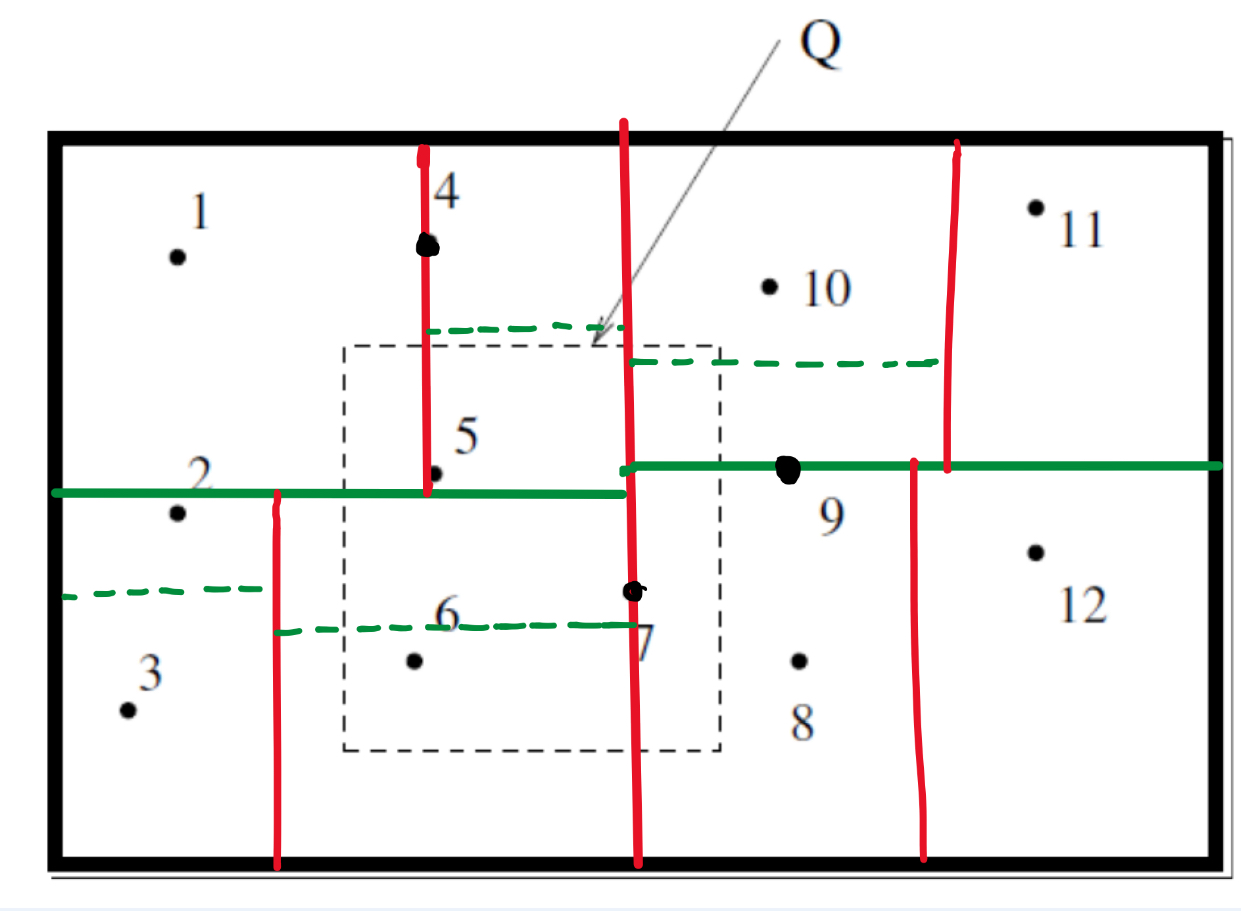
\includegraphics[width=\textwidth]{Images/kd.jpg}
         \caption{Partition of the plane }
         \label{fig:kd}
     \end{subfigure}
     
     \begin{subfigure}[b]{0.45\textwidth}
         \centering
         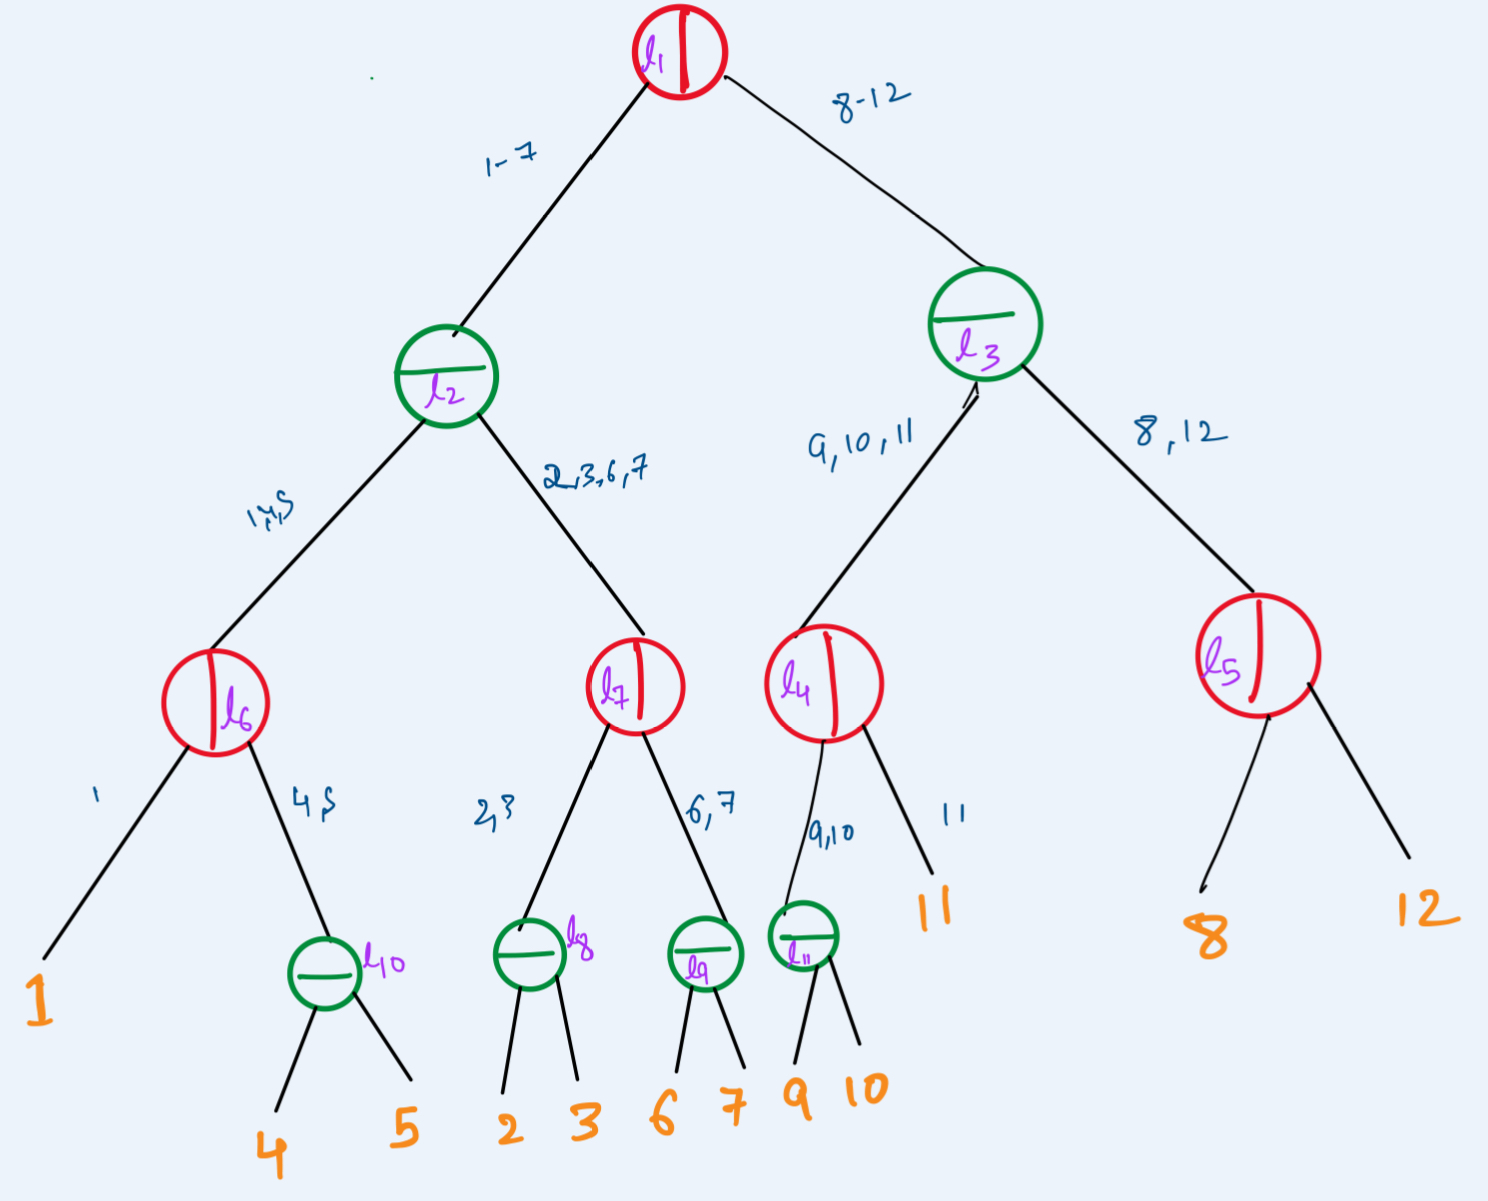
\includegraphics[width=\textwidth]{Images/kdinit.jpg}
         \caption{Initial kd-tree construct}
         \label{fig:kdinit}
     \end{subfigure}
    \hfill
     \begin{subfigure}[b]{0.5\textwidth}
         \centering
         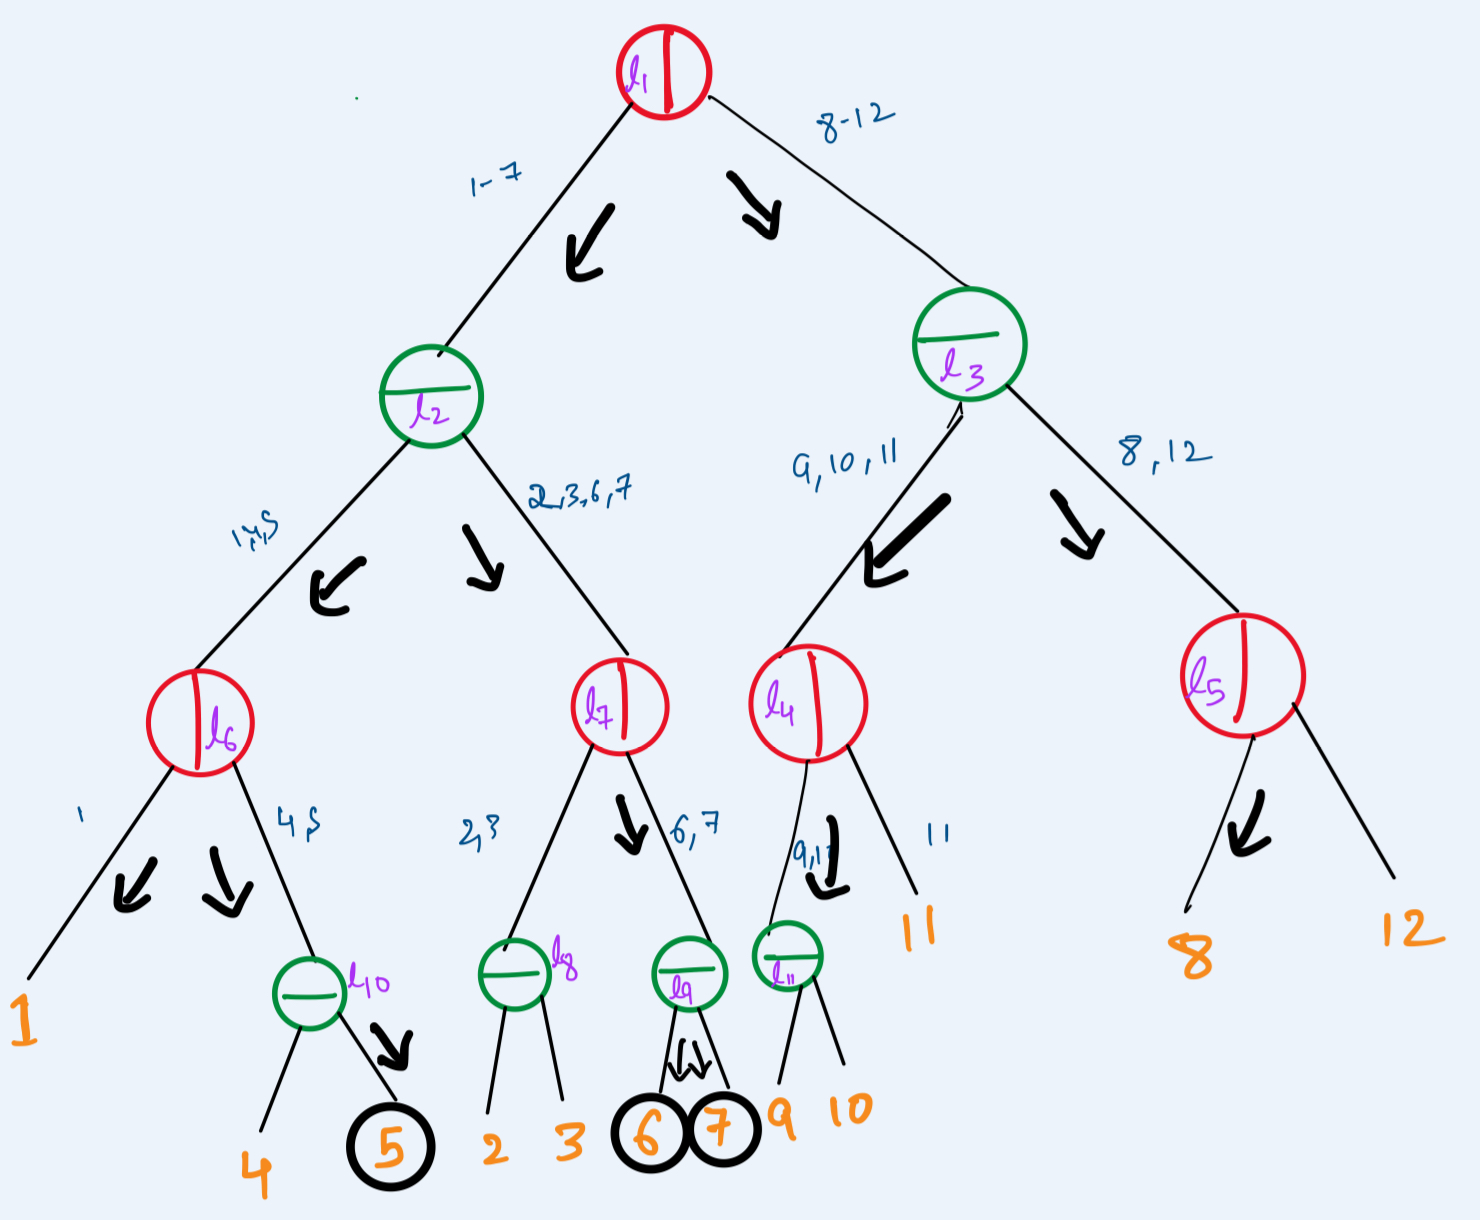
\includegraphics[width=\textwidth]{Images/kdfin.jpg}
         \caption{Corresponding y-range tree of I}
         \label{fig:kdfin}
     \end{subfigure}
        \caption{(b) Shows initial kd-tree. Horizontal lines are shown in green whereas vertical are shown in red. Also the corresponding partition of the plane is as shown in \Cref{fig:kd}.(c) Shows how the points contained in a query rectangle $Q$ can be returned given the location of Q and its dimensions. Black arrows show the nodes visited during the search. Leaf nodes finally found inside the given query range $Q$ are marked around in black circles.}
        \label{fig:kdall}
\end{figure}


Next, \Cref{fig:kdfin} shows how the points contained in a query rectangle $Q$ can be returned given the location of Q and its dimensions. Black arrows show the nodes visited during the search. Leaf nodes finally found inside the given query range $Q$ are marked around in black circles.

Directly following from the lectures, the \textbf{construction} takes \textbf{$\bm{O(nlogn)}$ time} (sorting w.r.t x and y-coordinates) and \textbf{$\bm{O(n)}$ space} (for storing the tree with $O(n)$ nodes) where as the \textbf{query} complexity is $\bm{O(\sqrt{n}+k)}$ where $k$ is the number of points reported inside $Q$.

\subsection{2D Range Tree}
\Cref{fig:2dinit} shows the problem formulated in terms of 2D range tree. To avoid any ambiguity in reading the image provided in the input, \Cref{fig:2dinit} also shows an array of points in increasing x-coordinates.


Next, \Cref{fig:2dfin} shows how we first search in the x-range of query $Q$. Black arrows show the nodes visited during the search. Subtrees finally found inside the given x-range of query $Q$ are marked around in black region. We here get two subtrees (numbered as in figure). For subtree II we do not show any corresponding y-range tree as it has only one node (here we directly conclude that the single point i.e. $6$, lies in the y-range of $Q$). For subtree-I, \Cref{fig:2dy} depicts the corresponding y-range tree for the nodes in the sub tree. We again search this y-range tree with y-range of $Q$ and traverse the tree (shown with black arrows).  Leaf nodes finally found inside the given query range $Q$ are marked with black ticks.


\begin{figure}[H]
     \centering
     \begin{subfigure}[b]{0.45\textwidth}
         \centering
         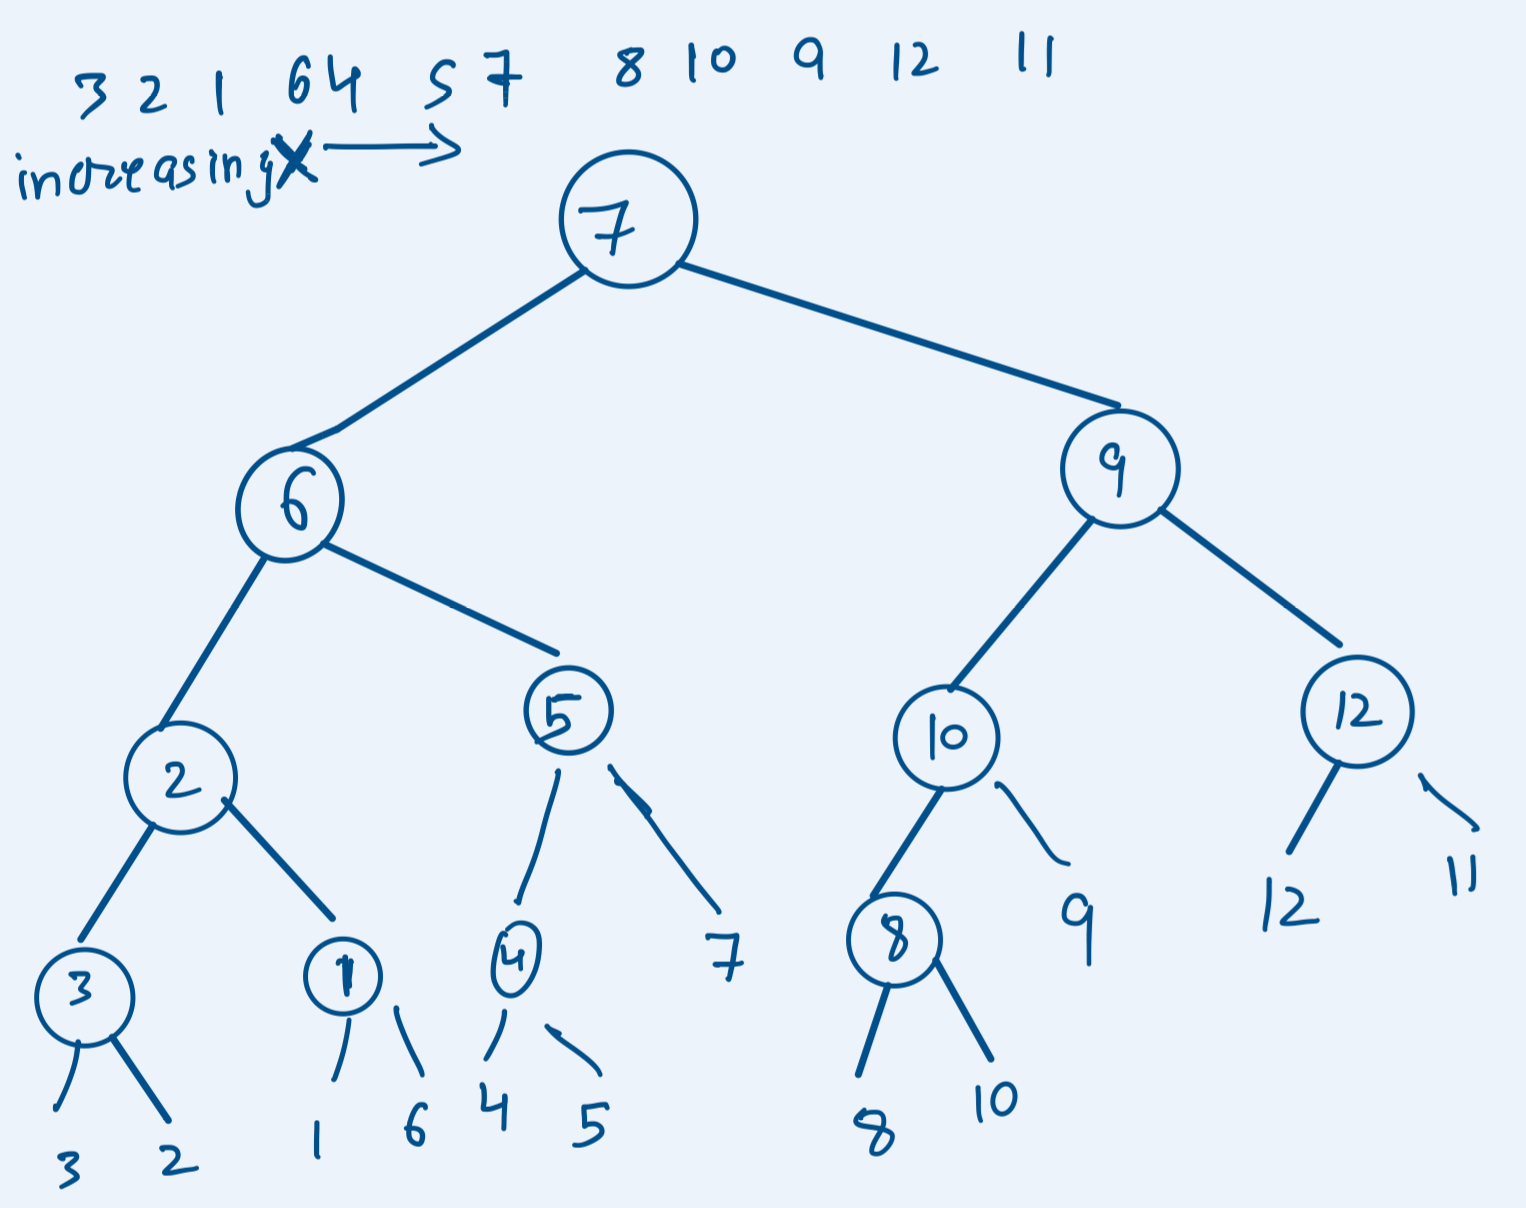
\includegraphics[width=\textwidth]{Images/2dinit.jpg}
         \caption{Initial x-range Tree}
         \label{fig:2dinit}
     \end{subfigure}
     \hfill
     \begin{subfigure}[b]{0.45\textwidth}
         \centering
         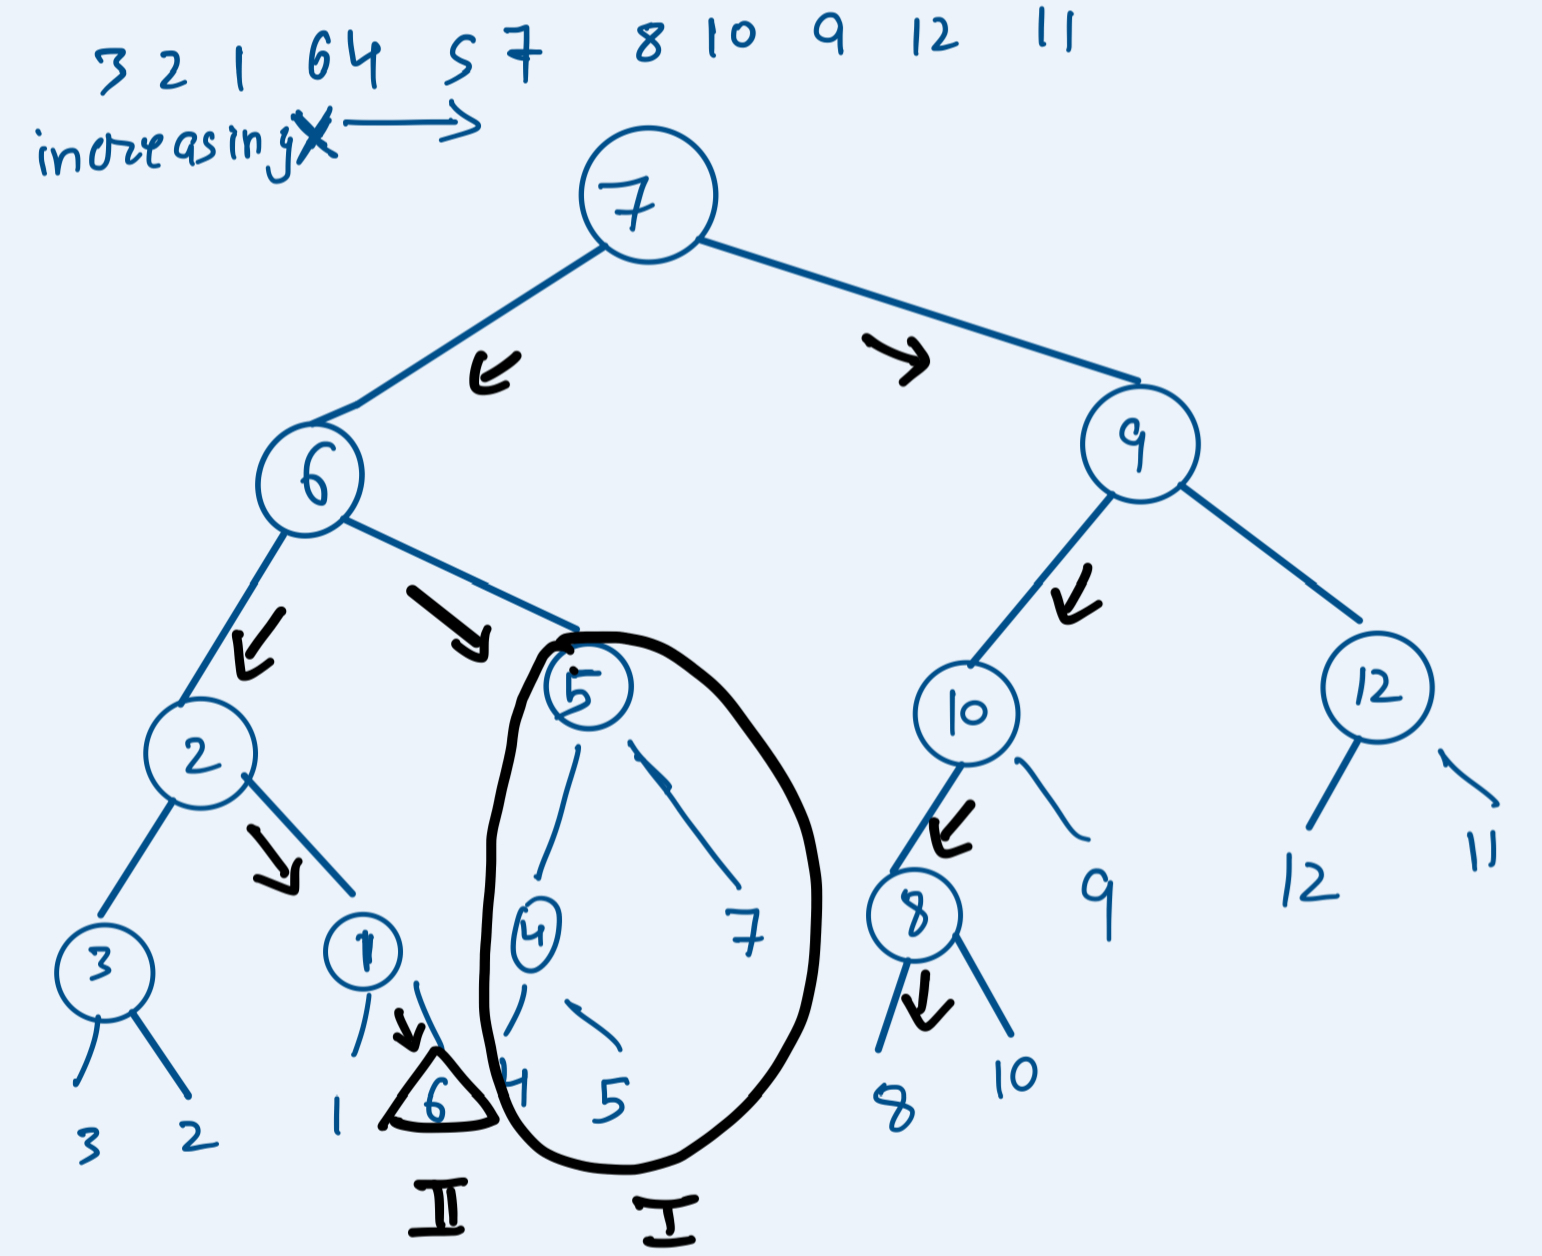
\includegraphics[width=\textwidth]{Images/2dfin.jpg}
         \caption{Search in the x-range of query}
         \label{fig:2dfin}
     \end{subfigure}

     \begin{subfigure}[b]{0.5\textwidth}
         \centering
         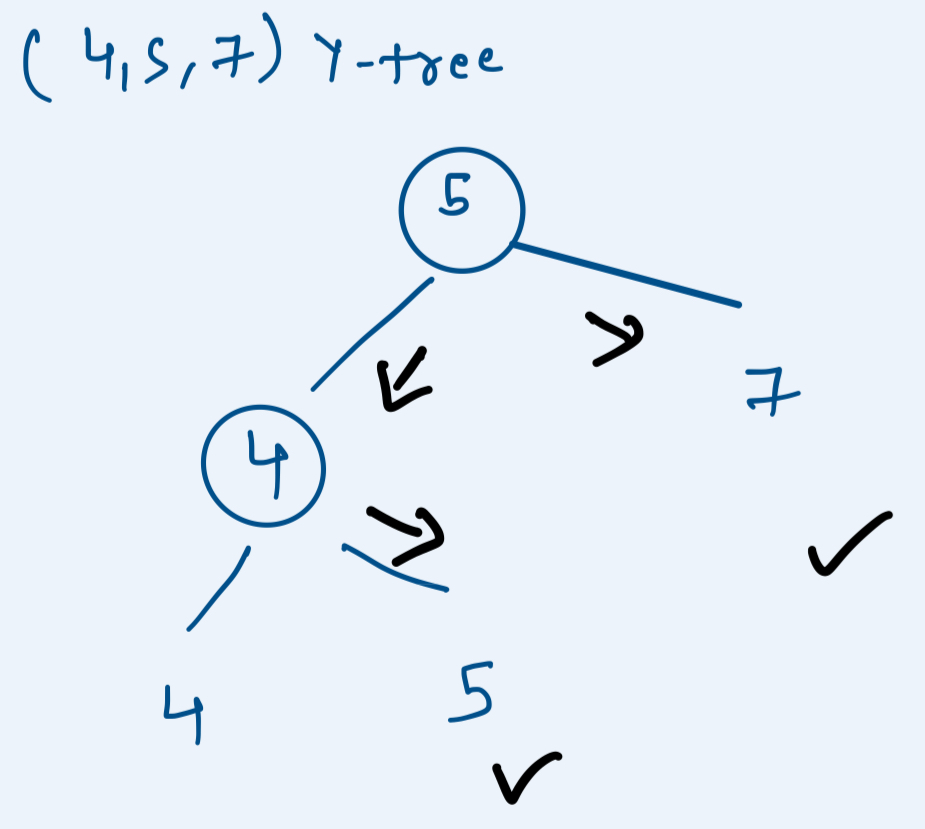
\includegraphics[width=\textwidth]{Images/yfin.jpg}
         \caption{Corresponding y-range tree of I}
         \label{fig:2dy}
     \end{subfigure}
        \caption{(a) Intial 2D Range tree construct. (b) Shows search in the x-range of query $Q$. Black arrows show the nodes visited during the search. Subtrees finally found inside the given x-range of query $Q$ are marked around in black region. Two subtrees are numbered as in figure. (b) Depicts the corresponding y-range tree for the nodes in the sub tree. We again search this y-range tree with y-range of $Q$ and traverse the tree (shown with black arrows).  Leaf nodes finally found inside the given query range $Q$ are marked with black ticks.}
        \label{fig:three graphs}
\end{figure}

Directly following from the lectures, the \textbf{construction} takes $\bm{O(nlogn)}$ \textbf{time} (sorting w.r.t x and y-coordinates) and $\bm{O(nlogn)}$ \textbf{space} (for storing $O(n)$ size x-tree and $O(n+\frac{n}{2}+\frac{n}{4}+..)=O(nlogn)$ size y-tree) where as the \textbf{query} complexity is $\bm{O(log^2{n}+k)}$ (with the use of fractional cascading, this can furhter be improved to $O(logn+k)$). where $k$ is the number of points reported inside $Q$.

\newpage
